\documentclass[a4paper, 12pt, oneside]{book}
\usepackage[italian]{babel} % Lingua italiana
\usepackage{authblk} % Per gli autori

\renewcommand\Authands{ e }

\title{Analisi empirica degli algoritmi di ordinamento}

\author[ ]{Graziano Francesco \thanks{Email: graziano.francesco@spes.uniud.it, Matricola: 166680}}
\author[ ]{Ongaro Michele \thanks{Email: ongaro.michele@spes.uniud.it, Matricola: 168049}}
\author[ ]{Petri Riccardo \thanks{Email: petri.riccardo@spes.uniud.it, Matricola: 167623}}
\author[ ]{Ungaro Marco \thanks{Email: ungaro.marco@spes.uniud.it, Matricola: 168934}}

\affil[ ]{Università degli Studi di Udine, Dipartimento di Matematica e Informatica}

\date{A.A. 2024-2025}
%\date{}

\usepackage{amsmath} % Per equazioni avanzate
\usepackage{amssymb} % Simboli matematici
\usepackage{graphicx} % Per immagini
\usepackage{lmodern} % Font simile a Computer Modern
\usepackage{geometry} % Per margini personalizzati
\usepackage{listings} % scrivere codice
\usepackage{float} % Per il posizionamento delle immagini

\geometry{a4paper, margin=2.5cm}
\cleardoublepage

\begin{document}

\renewcommand{\contentsname}{Contenuti}
\renewcommand{\chaptername}{Capitolo}

\maketitle % copertina del documento
\tableofcontents % sommario di tutti i titoli

\chapter{Introduzione}\label{chap:Introduzione} % (fold)

Il progetto richiede l'implementazione di quattro algoritmi di ordinamento per array di interi di dimensione variabile.
Gli algoritmi che andremo ad analizzare sono il Counting Sort, il Quick Sort, il Quick Sort 3 way e il Radix Sort (algoritmo a scelta).
Oltre alla corretta implementazione viene richiesto di effettuare un'analisi empirica dei tempi di esecuzione degli algorimti al variare della dimensione dell'array e del range dei valori interi. Per stimare i tempi di esecuzione di questi algoritmi garanantendo un errore relativo massimo pari a 0.001 adotteremo le seguenti metodologie:

\begin{itemize}
    \item Utilizzeremo un clock di sistema monotono per garantire precisione nelle misurazioni (ad esempio, \texttt{perf\_counter()} del modulo \(time\) in Python);
    \item Andremo a generare 100 campioni per ciascun grafico, con i valori dei parametri (dimensione dell'array \(n\) e intervallo dei valori \(m\)) distribuiti secondo una progressione geometrica;
    \item Effettueremo più esecuzioni per ogni campione, per stimare in modo affidabile il tempo medio di esecuzione.
\end{itemize}

\noindent Dopo aver stimato i tempi di esecuzione per ciascun algoritmo, risulterà interessante confrontare i grafici ottenuti per analizzarne il comportamento. 

% chapter Introduzione (end)


 
\chapter{Counting Sort}\label{chap:Counting Sort} % (fold)



% questa parte serve?
% da qui
Il Counting Sort è un algoritmo di ordinamento non comparativo: anziché effettuare confronti tra gli elementi, si basa sul conteggio delle occorrenze di ciascun elemento presente nell'array da ordinare.
È particolarmente efficiente quando gli elementi da ordinare sono numeri interi compresi in un intervallo limitato (intervallo \([0, k]\)).
L'implementazione adottata si articola in tre fasi principali:

\begin{itemize}
    \item Conteggio delle occorrenze di ciascun elemento; si costruisce un array ausiliario \(C\) di lunghezza \(k+1\), inizializzato a zero, in cui per ogni elemento \(x\) in \(A\), si incrementa \(C[x]\) di 1.
    \item Calcolo delle posizioni cumulative; per ottenere la posizione finale di ciascun elemento nell'array ordinato, si trasforma \(C\) in un array cumulativo. In questa versione, \(C[0]\) viene inizialmente decrementando di uno, così che \(c[i]\) rapprsenti l'indice massimo in cui si può inserire l'elemento \(i\) nell'array ordinato.
    \item Costruzione dell'array ordinato; si scorre l'array originale da destra a sinistra, e si inserisce ciascun elemento \(x\) nella posizione \(C[x]\) dell'array ordinato, decrementando \(C[x]\) di 1 dopo ogni inserimento. Questo garantisce la stabilità dell'ordinamento, poiché gli elementi con lo stesso valore vengono inseriti nell'ordine in cui appaiono nell'array originale.
\end{itemize}
% a qui

\noindent Le due funzioni fornite nel codice sono:

\begin{itemize}
    \item \texttt{countingSort(A, B, k)}: modifica il vettore B scrivendoci all'interno l'ordinamento crescente di A;
    \item \texttt{uniformedCountingSort(A, k)}: funzione wrapper che restituisce direttamente una copia ordinata di A.
\end{itemize}

\section{Analisi della complessità}

% serve davvero
% da qui
Siano \(n\) la dimensione dell'array \(A\) e \(k\) il valore massimo contenuto in \(A\). \\

\noindent \textbf{Tempo:}

\begin{itemize}
    \item Conteggio: \(O(n)\) per scorrere l'array \(A\) e contare le occorrenze di ciascun elemento.
    \item Calcolo delle posizioni cumulative: \(O(k)\) per trasformare l'array \(C\) in un array cumulativo.
    \item Costruzione dell'array ordinato: \(O(n)\) per scorrere l'array \(A\) e inserire gli elementi nell'array ordinato \(B\).
    \item Totale: \(O(n + k)\).
\end{itemize}

\noindent \textbf{Spazio:}

\begin{itemize}
    \item Array ausiliario \(C\): richiede \(O(k)\) spazio.
    \item Array ordinato \(B\): richiede \(O(n)\) spazio.
    \item Totale: \(O(n + k)\).
\end{itemize}

\noindent L'algoritmo è efficiente quando \(k = O(n)\), ovvero quando il range massimo dei valori interi è proporzionale alla dimensione dell'array.
In scenari in cui \(k \gg n\), il costo della fase di conteggio e l'allocazione dell'array ausiliario \(C\) possono rendere l'algoritmo meno competitivo rispetto ad altri metodi di ordinamento.
% a qui


\section{Analisi empirica}

Sono stati condotti due esperimenti distinti per analizzare le prestazioni empiriche del Counting Sort:

\begin{itemize}
    \item Nel primo esperimento, la dimensione dell'array \(n\) varia, mentre il valore massimo \(k\) è mantenuto fisso a 100000.
    \item Nel secondo esperimento, \(n\) è fissato a 10000, e viene fatto variare \(k\).
\end{itemize}

\noindent In entrambi i casi, i parametri sono stati scelti seguendo una progressione geometrica.
Per ogni valore di \(n\) o \(m\) sono stati generati 100 campioni casuali, ciascuno eseguito più volte per stimare in modo affidabile il tempo medio di esecuzione, mantenendo un errore relativo massimo \(\leq\) 0.001.
Le misurazioni sono state effettuate utilizzando un clock monotono ad alta precisione (\texttt{time.perf\_counter()} in Python). \\

\subsection{Primo esperimento ($n$ varia)}

\noindent
In primo luogo, è stato analizzato l'andamento temporale al variare della dimensione dell'array \(n\), mantenendo costante l'intervallo dei valori a \(k = 100000\). 
Il grafico seguente mostra in:
\begin{itemize}
    \item \textbf{Ascissa}: dimensione \(n\) dell'array;
    \item \textbf{Ordinata}: tempo di esecuzione per l'ordinamento espresso in secondi.
\end{itemize}

\begin{figure}[H]
    \centering
    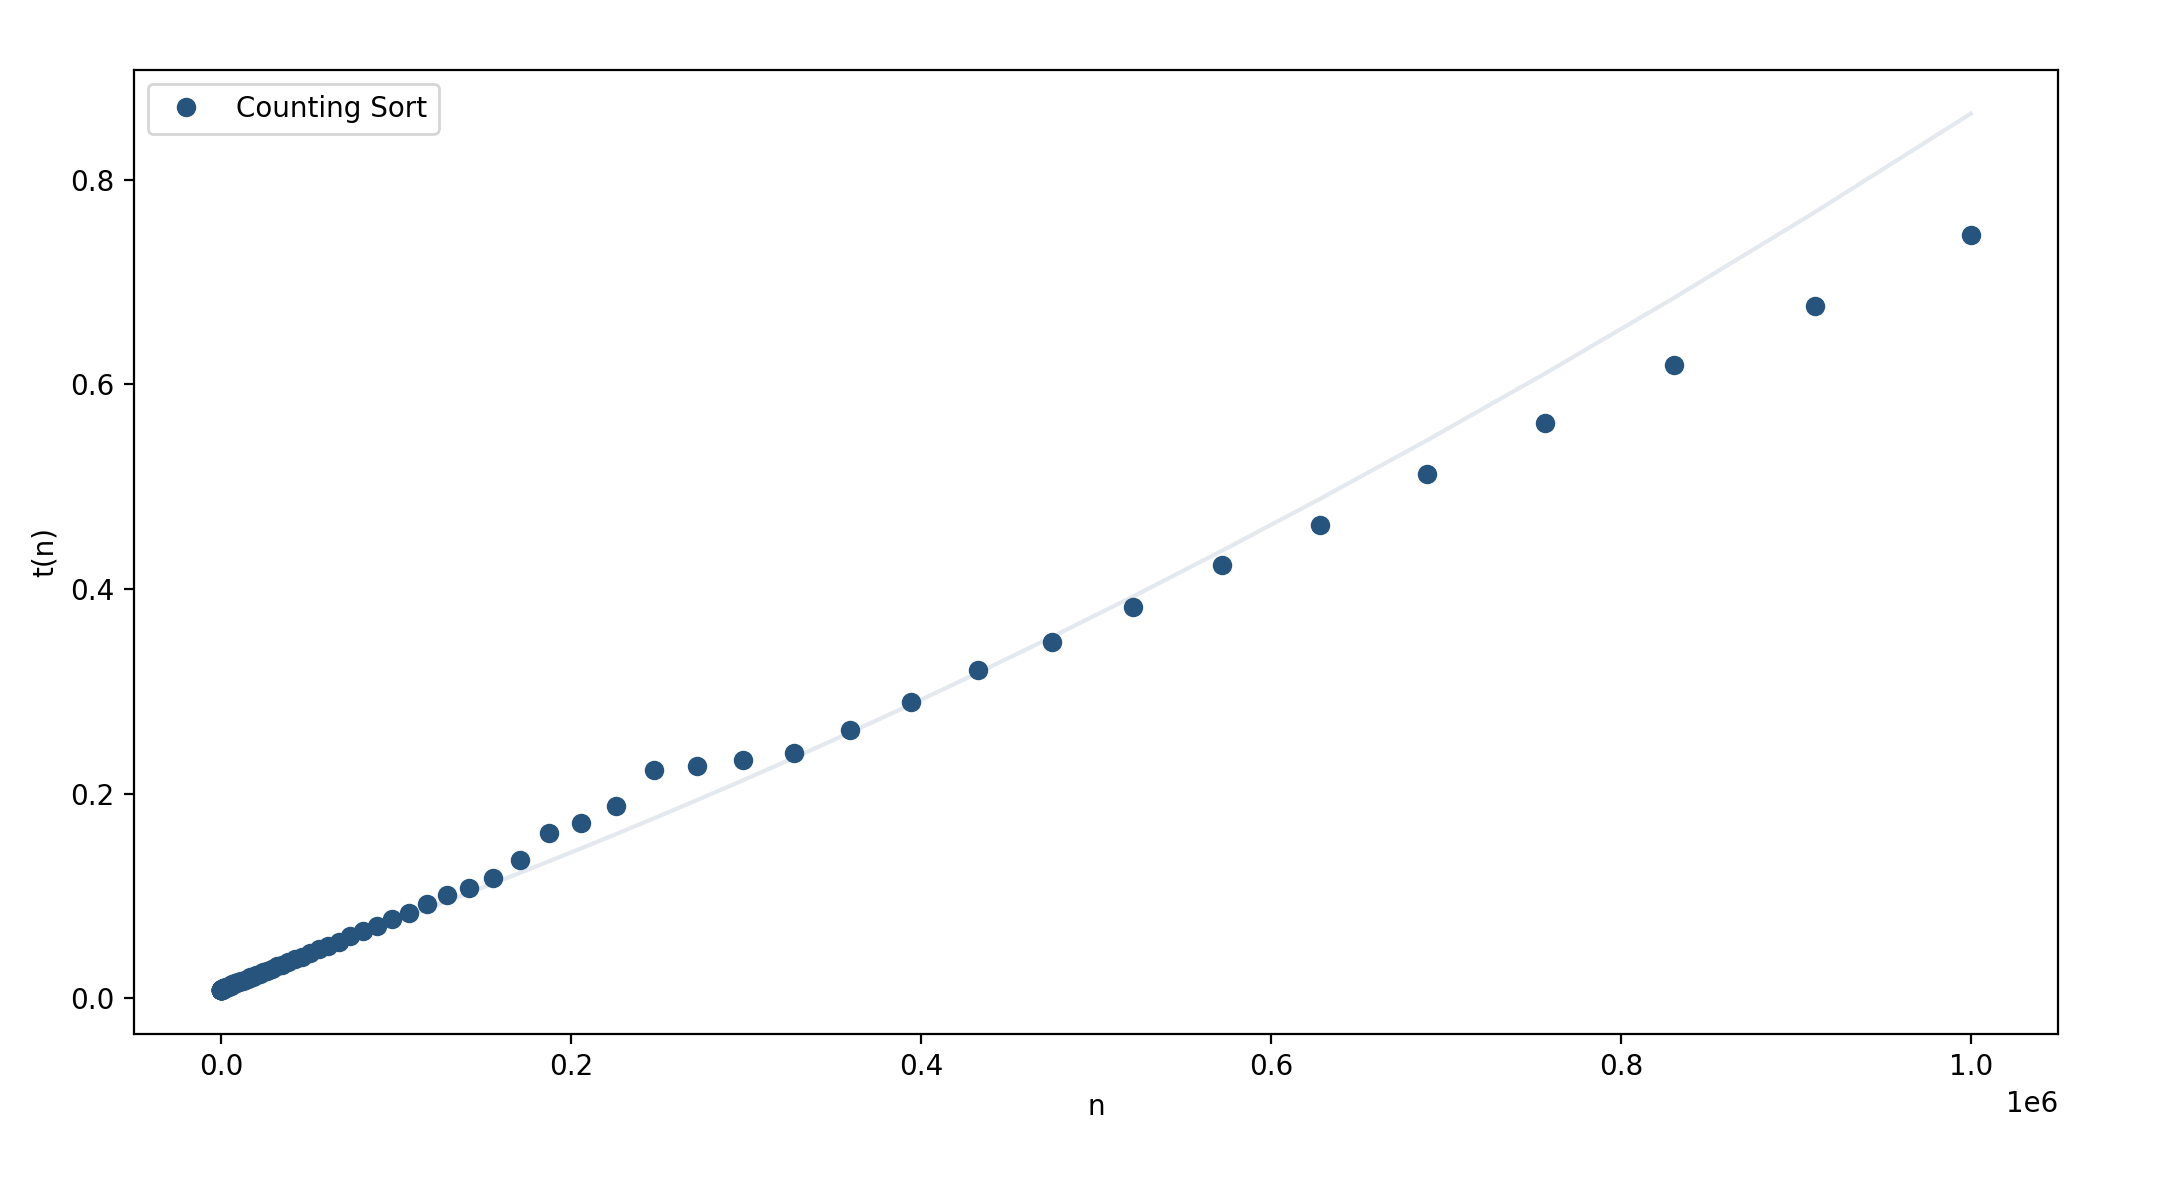
\includegraphics[width=0.8\textwidth]{images/grafico_counting_sort_n.png}
    \caption{Performance del Counting Sort al variare di \(n\).}
    \label{fig:counting_sort_n}
\end{figure}

\subsection{Secondo esperimento ($m$ varia)}

\noindent Successivamente, è stato analizzato l'andamento temporale al variare dell'intervallo di valori \(m\), mantenendo costante la dimensione dell'array a \(n = 10000\). 
Il grafico seguente presenta:
\begin{itemize}
    \item \textbf{Ascissa}: intervallo \(m\) dei valori;
    \item \textbf{Ordinata}: tempo di esecuzione per l'ordinamento espresso in secondi.
\end{itemize}

\begin{figure}[H]
    \centering
    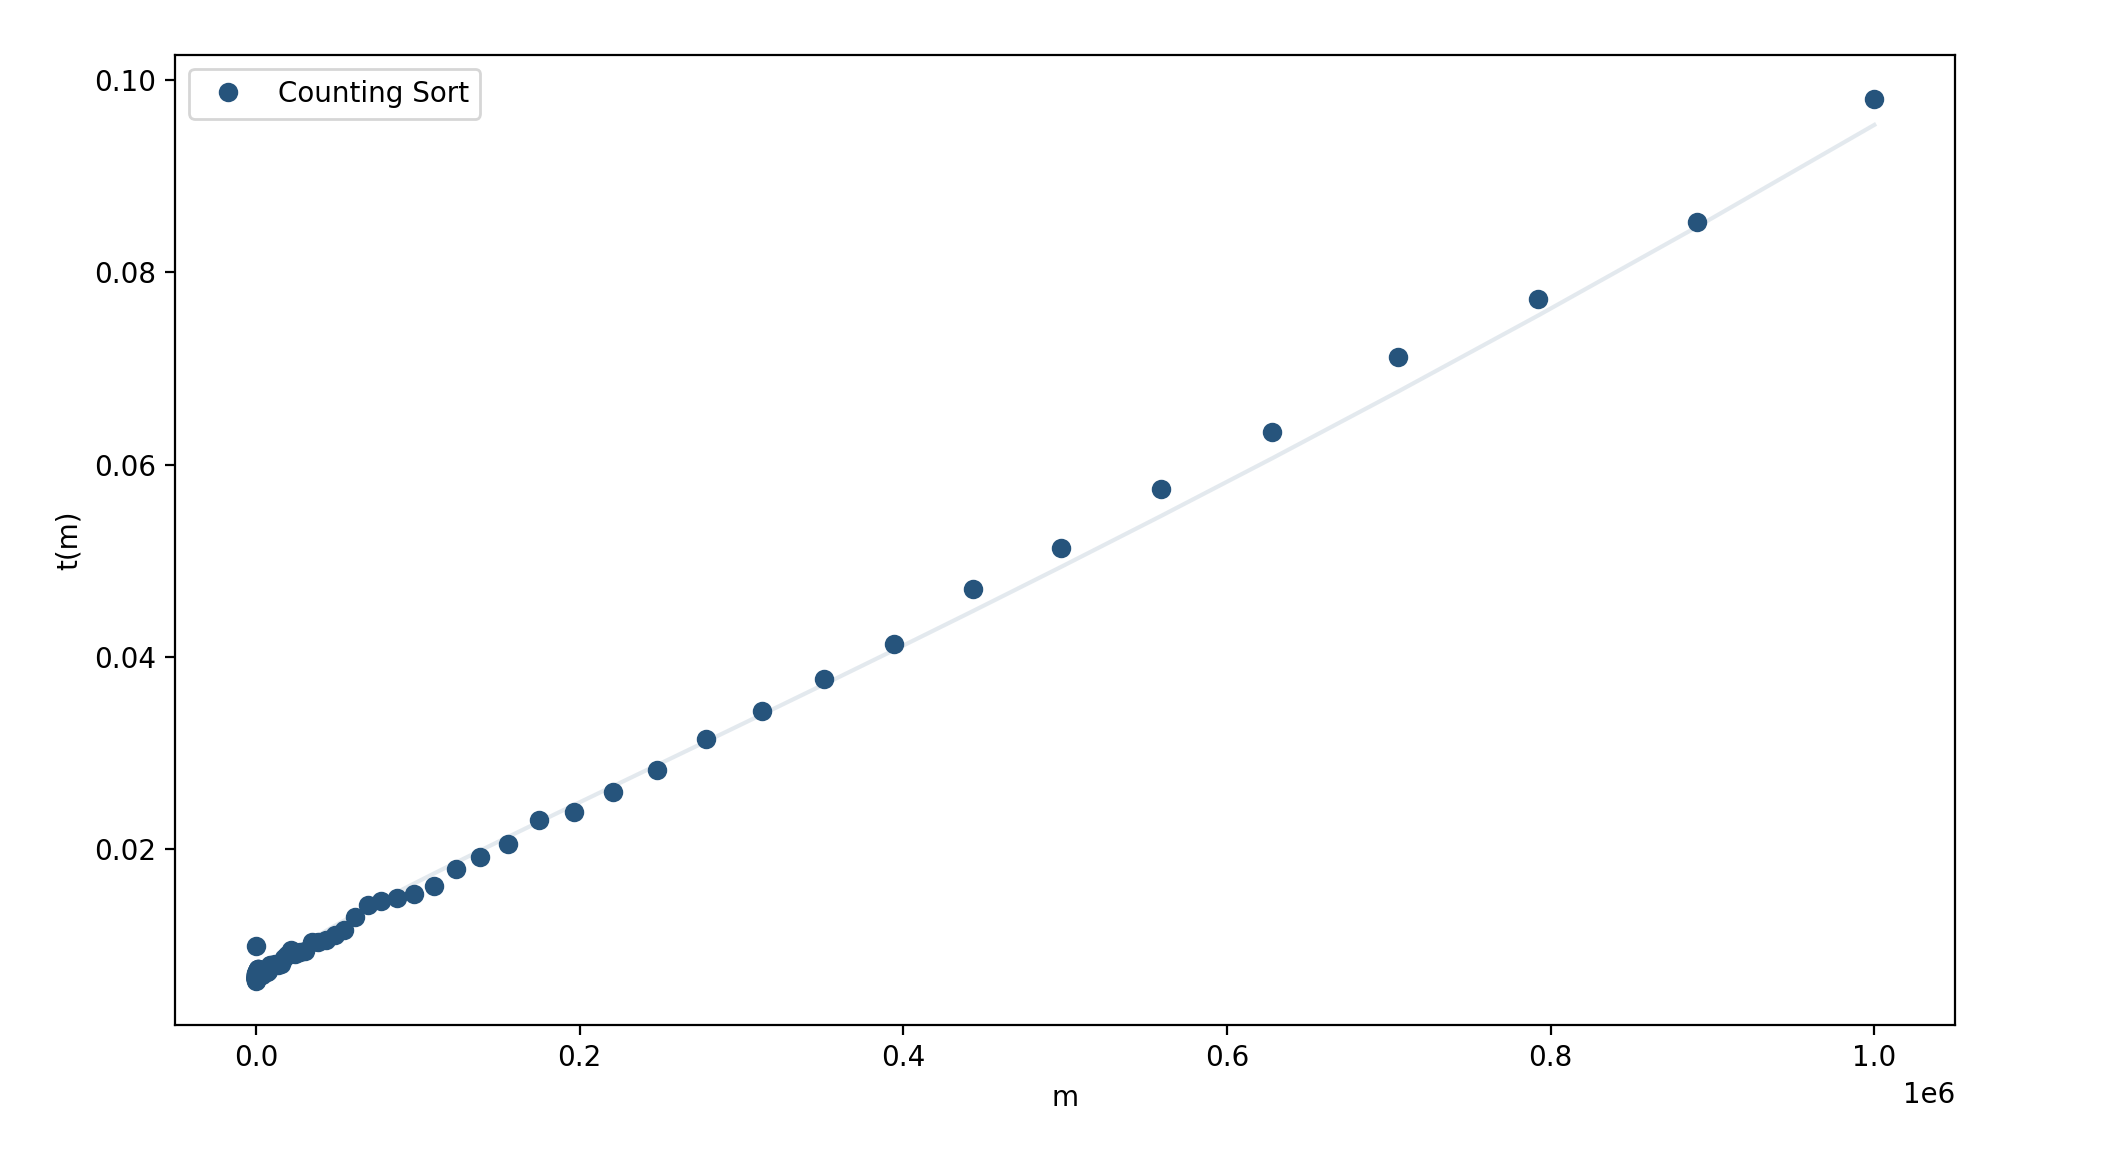
\includegraphics[width=0.8\textwidth]{images/grafico_counting_sort_m.png}
    \caption{Performance del Counting Sort al variare di \(m\).}
    \label{fig:counting_sort_m}
\end{figure}

% chapter Counting Sort (end)

\chapter{Quick Sort}\label{chap:Quick Sort} % (fold)

% serve davvero?
% da qui
Il Quick Sort è un algoritmo di ordinamento basato sulla strategia del divide et impera (ovvero: dividere il problema in sottoproblemi più piccoli, risolverli ricorsivamente e combinare i risultati).
A partire da un array \(A\), si seleziona un pivot, in questo caso l'elemento finale del sottoarray \(A[p...q]\), e si procede alla partizione: tutti gli elementi minori o uguali al pivot vengono spostati a sinistra, quelli maggiori a destra. L'indice finale del pivot è restituito dalla funzione partition, e l'algoritmo viene poi richiamato ricorsivamente sulle due sottosequenze risultanti.
% a qui?


\noindent Le due funzioni fornite nel codice sono:

\begin{itemize}
    \item \texttt{quicksort(A, p, q)}: aggiorna il contenuto del vettore A ordinandolo dal range da $p$ a $q$;
    \item \texttt{uniformedQuickSort(A, k)}: funzione wrapper per rendere uniforme l'interfaccia tra gli algoritmi testati che esegue l'algoritmo Quick Sort sull'intero vettore A.
\end{itemize}

\noindent
L'implementazione del Quick Sort analizzata non è in place a causa della coda delle ricorsioni, e non soddisfa la condizione di stabilità.

\section{Analisi della complessità}

Sia \(n\) la dimensione dell'array da ordinare:

\begin{itemize}
    \item Caso medio: \(O(n \cdot log(n))\), si verifica quando il pivot divide l'array in modo bilanciato.
    \item Caso migliore: \(O(n \cdot log(n))\), con partizioni esattamente simmetriche.
    \item Caso peggiore: \(O(n^2)\), quando il pivot è sempre il minimo o il massimo elemento (partizione altamente sbilanciata).
    \item Spazio ausiliario: \(O(log(n))\) nel caso medio per la profondità dello stack ricorsivo; \(O(n)\) nel caso peggiore.
\end{itemize}

\noindent A differenza di altri algoritmi come Counting Sort o Radix Sort, Quick Sort non richiede conoscenza del range dei valori interi e lavora unicamente tramite confronti tra elementi.

\section{Analisi empirica}

Per analizzare empiricamente il comportamento del Quick Sort sono stati eseguiti due esperimenti distinti:

\begin{itemize}
    \item Nel primo esperimento la dimensione dell'array \(n\) viene fatta variare, mantenendo fisso \(m = 100000\).
    \item Nel secondo esperimento abbiamo \(n = 10000\) costante, con variazione di \(m\).
\end{itemize}

\noindent In entrambi i casi, i parametri sono distribuiti secondo una progressione geometrica.
Per ogni coppia \((n, m)\) sono stati generati 100 campioni casuali, ciascuno eseguito più volte per stimare in modo accurato il tempo medio di esecuzione, con un errore relativo massimo \(\leq 0.001\).
Le misurazioni sono state effettuate mediante un clock monotono ad alta precisione (\texttt{time.perf\_counter()} in Python). \\

\noindent
Poiché Quick Sort opera esclusivamente tramite confronti, il valore massimo m non influisce direttamente sulla complessità. Tuttavia, può avere effetti indiretti sulla distribuzione dei dati (ad esempio, la presenza di molti duplicati o valori ripetuti), il che può influenzare l'efficienza della partizione. \\

\subsection{Primo esperimento ($n$ varia)}

A partire dai dati misurati è stato generato un grafico nel quale la lunghezza dell'array indicata con \(n\) varia da 100 a 1000000, mentre il parametro \(m\) (range dei valori) è mantenuto costante. L'ordinamento è stato eseguito utilizzando l'algoritmo Quick Sort su array contenenti numeri casuali.

\begin{figure}[H]
    \centering
    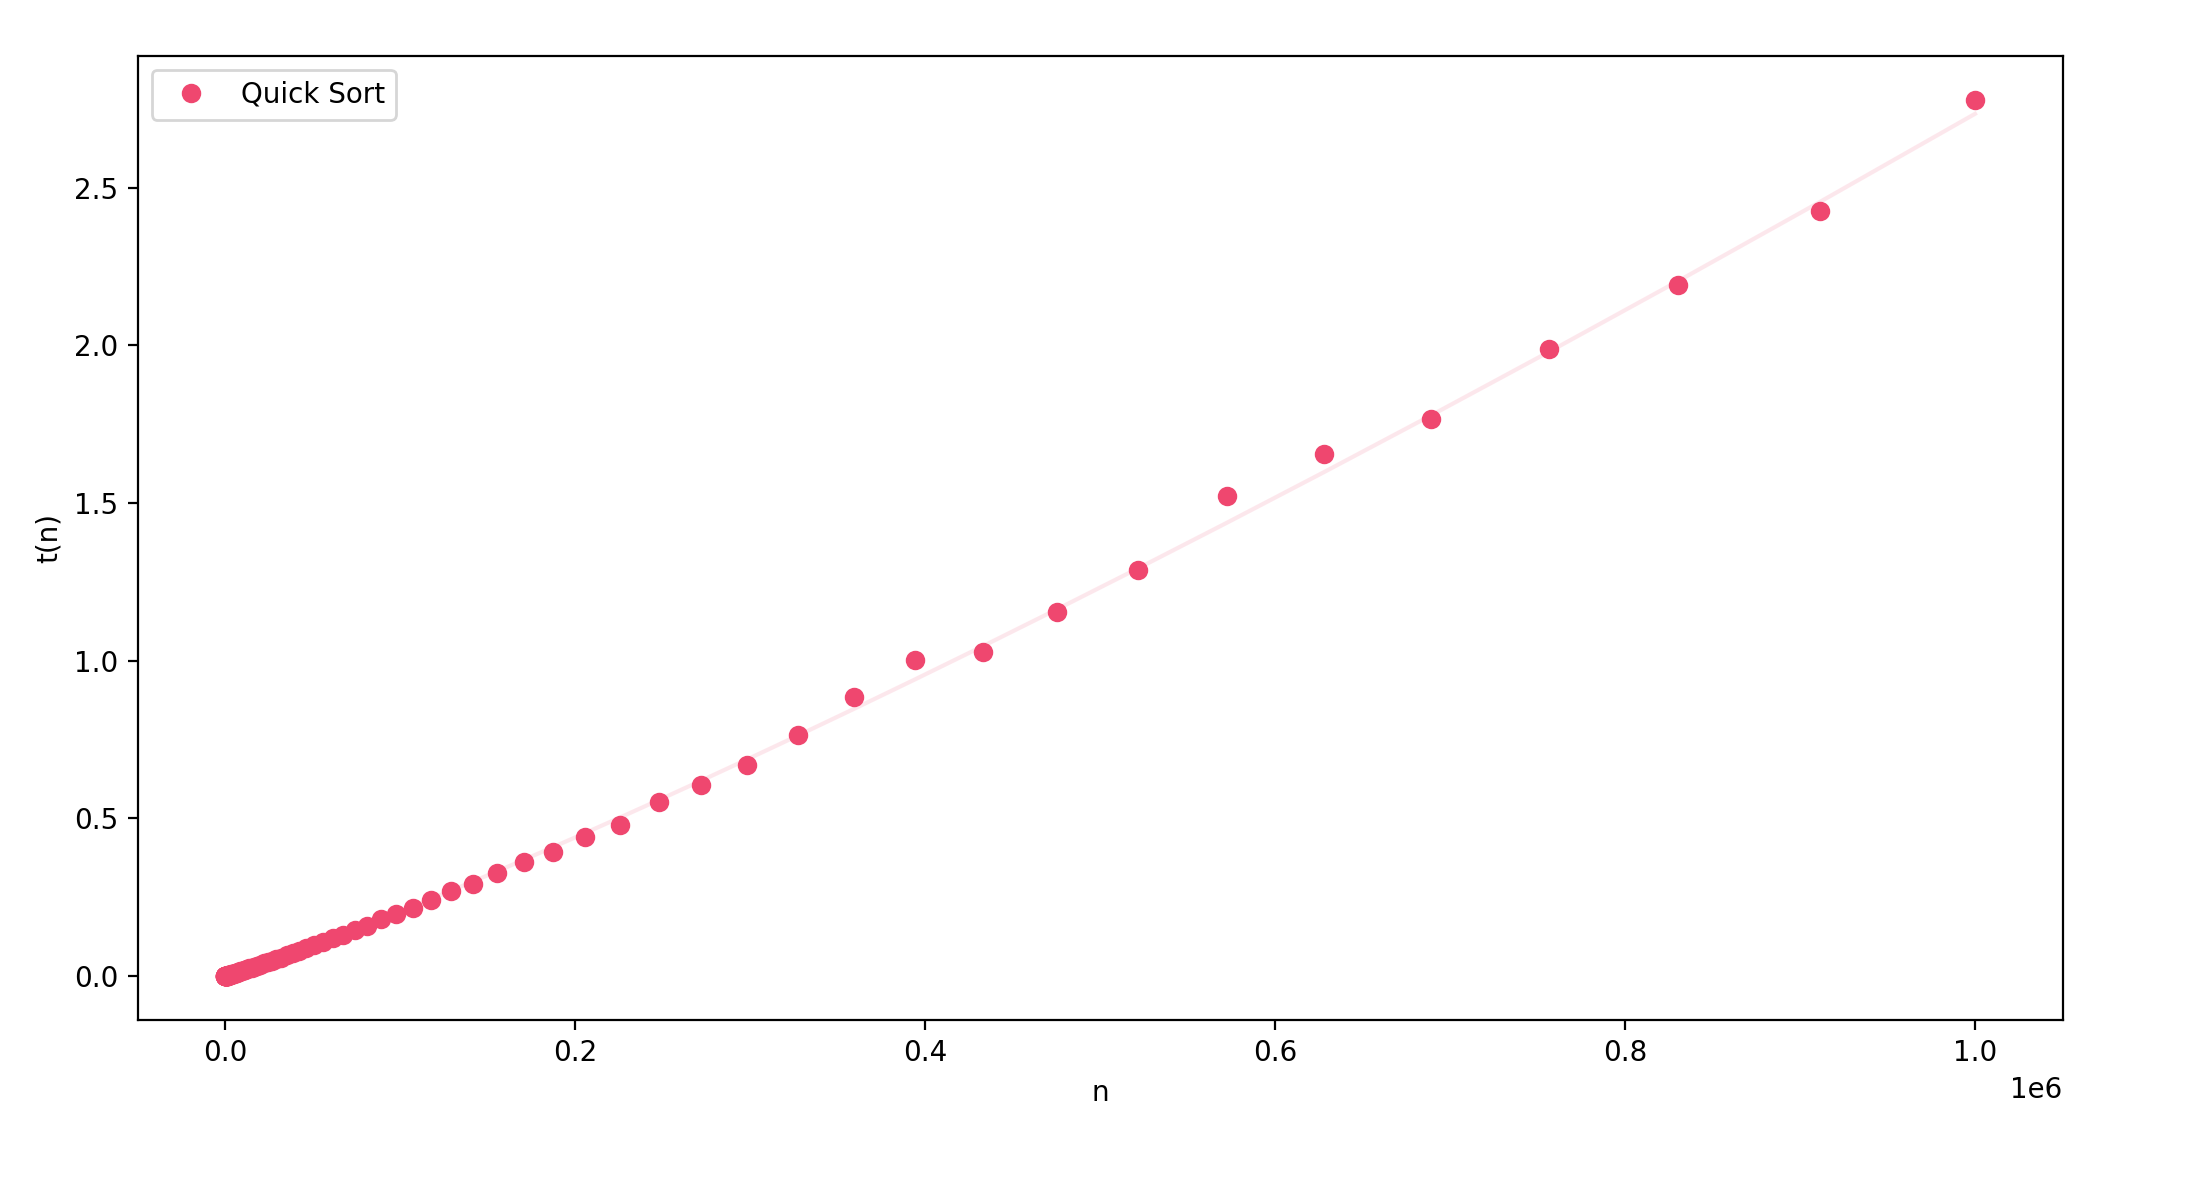
\includegraphics[width=0.8\textwidth]{images/grafico_quick_sort_n.png}
    \caption{Performance del Quick Sort al variare di \(n\).}
    \label{fig:quick_sort_n}
\end{figure}

\subsection{Secondo esperimento ($m$ varia)}

\noindent Successivamente, è stato realizzato un grafico in cui varia il range dei valori interi presenti nell'array, indicato con \(m\), mantenendo costante la dimensione dell'array a \(n=10000\). Nel grafico riportato di seguito, sull'asse delle ascisse è rappresentata la variazione di \(m\), da 10 a 1.000.000, in scala scientifica. Sull'asse delle ordinate è riportato il tempo medio di esecuzione dell'ordinamento, espresso in secondi.

\begin{figure}[H]
    \centering
    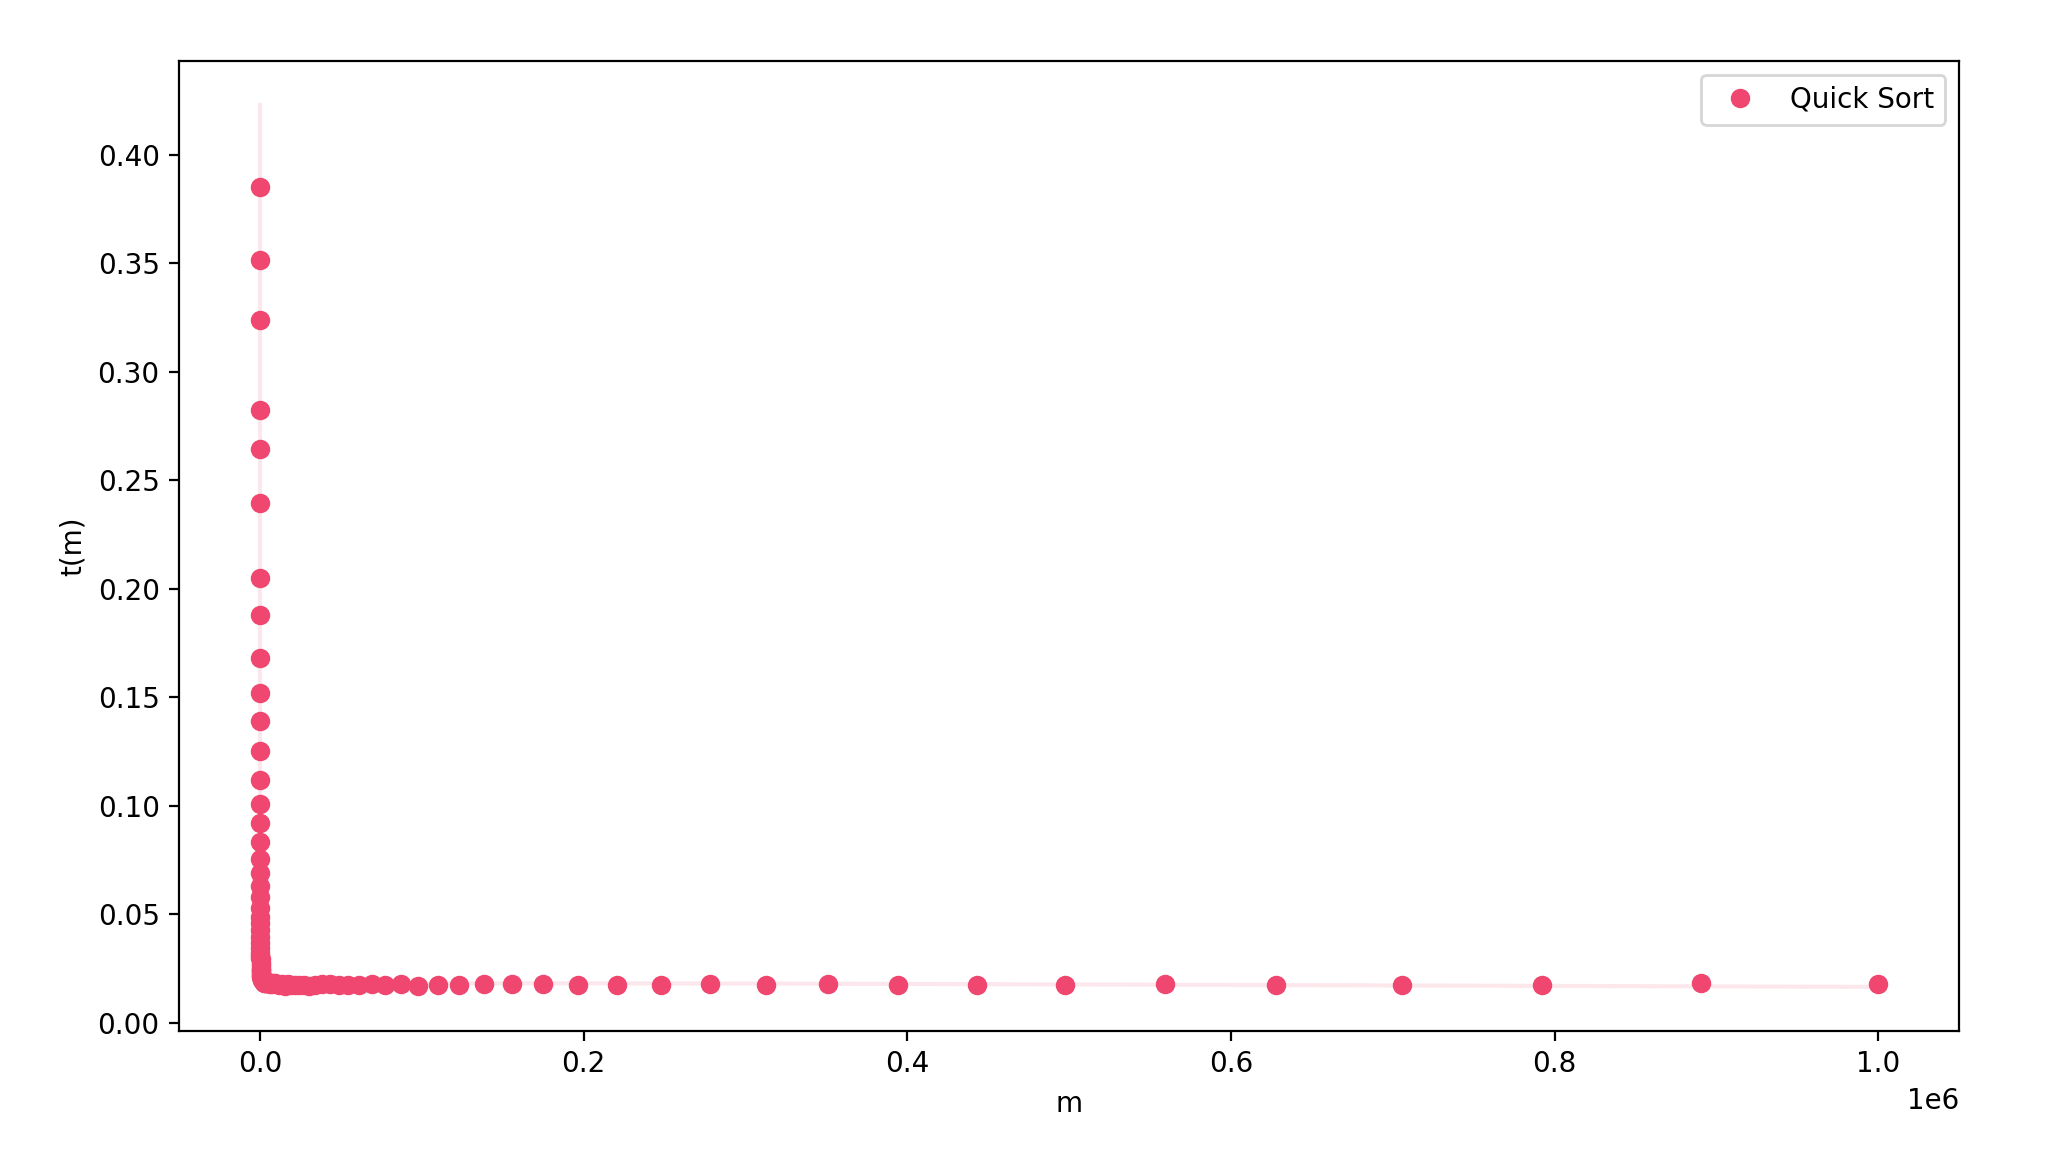
\includegraphics[width=0.8\textwidth]{images/grafico_quick_sort_m.png}
    \caption{Performance del Quick Sort al variare di \(m\).}
    \label{fig:quick_sort_m}
\end{figure}

\noindent Si osserva un'anomalia nel grafico quando il numero di valori distinti presenti nell'array (\(m\)) è molto basso. La motivazione è presto detta: Quick Sort rischia di diventare $O(n^2)$ se ci sono tante ripetizioni dello stesso elemento, cosa che, per il principio della piccionaia avviene per valori di $m$ piuttosto bassi (e.g. un'array da 10000 elementi che contiene elementi che possono assumere solamente 10 valori diversi risulta avere molte ripetizioni).

% chapter Quick Sort (end)

\chapter{Quick Sort 3 Way}\label{chap:Quick Sort 3 Way} % (fold)

Il Quick Sort 3-Way è una variante del Quick Sort classico, progettata per migliorare l'efficienza in presenza di molti elementi duplicati. Come il Quick Sort tradizionale, segue la strategia del divide et impera (cioè suddividere l'array in parti più semplici da ordinare ricorsivamente).
A differenza della versione classica, che suddivide in due partizioni (elementi minori o maggiori del pivot), il Quick Sort 3-Way suddivide l'array in tre sezioni distinte:

\begin{itemize}
    \item Elementi minori del pivot;
    \item Elementi uguali al pivot;
    \item Elementi maggiori del pivot.
\end{itemize}

\noindent Questa suddivisione viene effettuata durante la fase di partizionamento, evitando confronti e ricorsioni inutili sugli elementi uguali al pivot, che sono già in posizione corretta. La ricorsione viene infatti applicata solo alle sottosequenze strettamente minori o maggiori del pivot.
L'algoritmo è in-place (non richiede spazio addizionale significativo) ma non stabile (gli elementi uguali possono cambiare ordine relativo).

\section{Analisi della complessità}

Sia \(n\) la dimensione dell'array:

\begin{itemize}
    \item Caso migliore: \(O(n)\), quando tutti gli elementi sono uguali, e la partizione centrale include l'intero array.
    \item Caso medio: \(O(n \cdot log(n))\), come il Quick Sort classico, ma con una costante migliore grazie alla gestione efficiente dei duplicati.
    \item Caso peggiore: \(O(n^2)\), in caso di pivot molto sbilanciati e assenza di duplicati.
    \item Spazio ausiliario: \(O(log(n))\) per la profondità della ricorsione.
\end{itemize}

\noindent Nel complesso, Quick Sort 3-Way si comporta meglio del Quick Sort classico in presenza di dati con molti valori ripetuti, mantenendo lo stesso ordine di complessità.

\section{Analisi empirica}

Per verificare empiricamente l'efficienza dell'algoritmo, sono stati condotti due esperimenti separati:

\begin{itemize}
    \item Nel primo esperimento abbiamo \(m = 100000\) fisso, mentre la dimensione dell'array che varia da \(100\) a $100000$
    \item Nel secondo esperimento la dimensione dell'array è \(n = 10000\) mentre viene fatto variare il range dei valori \(m\) da $10$ a $1000000$.
\end{itemize}

I valori di \(n\) e \(m\) sono distribuiti secondo una progressione geometrica. Per ogni coppia di parametri sono stati generati almeno 100 campioni casuali, ciascuno eseguito più volte. I tempi medi di esecuzione sono stati stimati con un clock monotono ad alta precisione (\texttt{time.perf\_counter()}), garantendo un errore relativo massimo \(\leq 0.001\). \\

\noindent I risultati ottenuti sono coerenti con le aspettative teoriche:

\begin{itemize}
    \item Nel primo esperimento, i tempi crescono approssimativamente secondo una curva \(O(n \cdot log(n))\), come previsto.
    \item Nel secondo esperimento, si osserva che, riducendo \(m\), aumentano i duplicati nei dati, e l'algoritmo ne beneficia: i tempi di esecuzione diminuiscono sensibilmente grazie al partizionamento ottimizzato del Quick Sort 3-Way.
\end{itemize}

\noindent Nel grafico allegato si evidenziano chiaramente i vantaggi di questa variante rispetto alla versione classica, soprattutto in presenza di dati ridondanti.

% chapter Quick Sort 3 Way (end)

\chapter{Radix Sort}\label{chap:Radix Sort} % (fold)

Il Radix Sort è un algoritmo di ordinamento non comparativo che sfrutta le rappresentazioni numeriche degli elementi. Ordina i numeri interi cifra per cifra, a partire dalla cifra meno significativa (LSD - Least Significant Digit) fino a quella più significativa. L'ordinamento delle singole cifre è effettuato tramite un algoritmo stabile, come il Counting Sort, applicato in sequenza per ogni posizione.
Radix Sort lavora bene quando si conosce il numero massimo di cifre degli elementi (ovvero \(log_{10}(k)\) se \(k\) è il valore massimo presente).
Questo algoritmo è in-place (usa spazio aggiuntivo proporzionale a \(n + b\), con \(b\) la base usata, tipicamente \(10\)), ma non stabile per natura a meno che il sorting delle cifre lo sia (in questo caso è garantita la stabilità tramite Counting Sort).

\section{Analisi della complessità}
Sia \(n\) la lunghezza dell'array e \(d\) il numero massimo di cifre (ossia \( d = \lceil \log_{10}(k + 1) \rceil \)): \\

\begin{itemize}
    \item Tempo: \(O(d \cdot (n + b))\), che nel caso più comune (\(b = 10\)) diventa \(O(n \cdot log_{10}(k))\). Quando \(k = O(n^c)\) per una costante \(c\), si ha complessivamente tempo quasi-lineare \(O(n)\).
    \item Spazio: \(O(n + b)\) per ogni cifra, dove \(b\) è la base (es. 10 cifre decimali).
    \item Stabile: sì, se il counting sort interno è stabile.
    \item In-place: no, nel senso stretto (usa memoria ausiliaria \(O(n)\)).
\end{itemize}

\section{Analisi empirica}
L'algoritmo è stato testato su array di interi generati casualmente, secondo due configurazioni sperimentali:

\begin{itemize}
    \item Esperimento 1: \(m = 100000\) (valore massimo) fisso, variando la dimensione \(n\) dell'array.
    \item Esperimento 2: \(n = 10000\) fisso, variando \(m\), cioè il massimo valore presente negli elementi.
\end{itemize}

\noindent In entrambi i casi, i parametri sono scelti su una scala geometrica. Ogni configurazione \((n, m)\) è stata eseguita su almeno 100 campioni, ciascuno ripetuto più volte. I tempi di esecuzione sono stati misurati tramite un clock monotono con errore relativo massimo \(\leq 0.001\). \\

\noindent I risultati ottenuti confermano l'efficienza teorica:

\begin{itemize}
    \item In Esperimento 1, il tempo di esecuzione cresce linearmente con \(n\), confermando il comportamento \(O(n \cdot log_{10}(k))\), dato \(k\) fisso.
    \item In Esperimento 2, aumentando \(k\) (cioè il numero massimo di cifre \(d\)), si osserva un aumento graduale dei tempi dovuto alla crescita del numero di passaggi di counting sort, coerente con la complessità \(O(d \cdot n)\).
\end{itemize}

\noindent Radix Sort si dimostra particolarmente adatto per dataset numerici con intervallo limitato, risultando spesso più veloce di algoritmi comparativi come Quick Sort nei casi in cui \(k = O(n)\) o \(k << n^2\).

% chapter Radix Sort (end)

\chapter{Conclusioni}\label{chap:Conclusioni} % (fold)

TODO (?)

% chapter Conclusioni (end)

\end{document}
